\chapter{Programa}\label{cap:programa}

\section{Introdução}

Este capítulo descreve o programa desenvolvido para implementar o algoritmo de
controle proposto no capítulo~\ref{cap:modelagem}, bem como as APIs e programas
utilizados adicionalmente para possibilitar a execução de testes comparativos.

Na seção~\ref{sec:arq_prog} uma arquitetura simplificada do sistema de controle é apresentada.
Por sistema de controle, entenda-se o processo que vai desde a aquisição dos
dados da visão, planejamento e trasmissão dos comandos aos robôs.

Na seção~\ref{sec:minimax} uma implementação do algoritmo de controle conceitualizado no
capítulo~\ref{cap:modelagem} é apresentada.

Na seção~\ref{sec:pyroboime} o programa pyroboime é descrito.

Na seção~\ref{sec:metricas} são propostas métricas para comparar o algoritmo
proposto com o utilizado anteriormente.

\section{Arquitetura do programa}\label{sec:arq_prog}

Um modelo simplificado da arquitetura do sistema de controle utilizado no para
o desenvolvimento deste projeto é apresentado na figura~\ref{fig:arq_prog}.

\begin{figure}
  \centering
  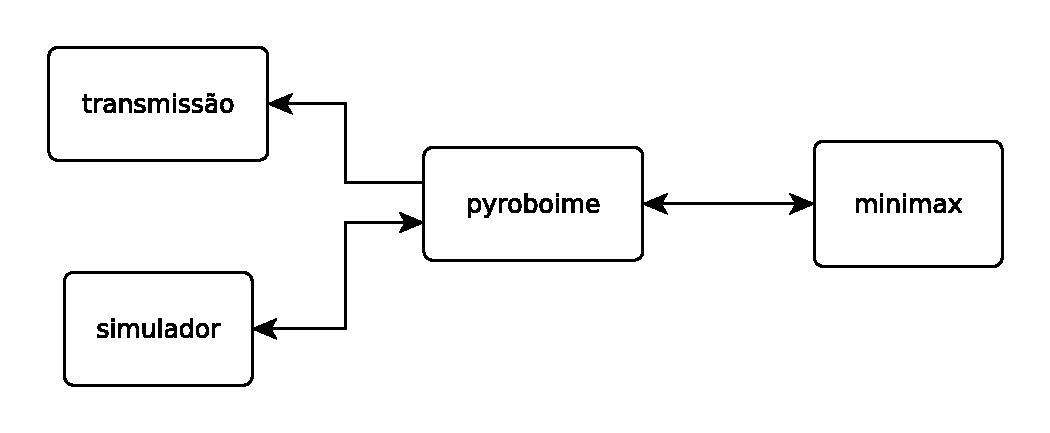
\includegraphics[width=0.8 \linewidth]{img/arq_geral_prog}
  \caption{Arquitetura simplificada do sistema de controle}\label{fig:arq_prog}
\end{figure}

\section{Processo do Minimax}\label{sec:minimax}

O fluxo do programa é apresentado na figura~\ref{fig:minimax_flow}.

\begin{figure}
  \centering
  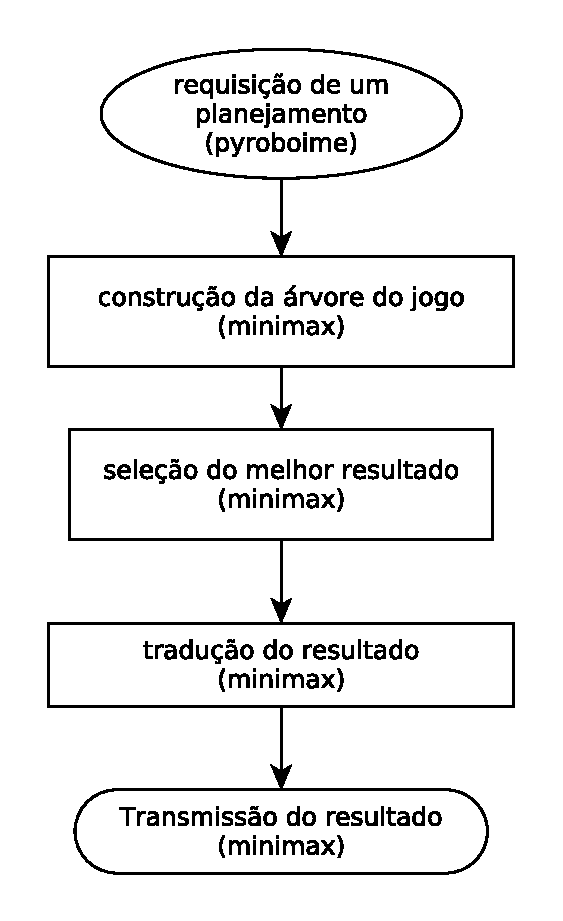
\includegraphics[width=0.2 \linewidth]{img/minimax_flow}
  \caption{Fluxo do processo minimax}\label{fig:minimax_flow}
\end{figure}

O processo de tradução consiste em transformar o planejamento obtido em uma
mensagem a ser enviada para o programa pyroboime. Para isso, foi utilizado
o protobuf. A estrutura do protocolo de resposta é apresentada no
arquivo~\ref{alg:minimax_resp_proto}. A estrutura do protocolo de atualização do
estado do tabuleiro apresentada no arquivo~\ref{alg:minimax_req_proto}.

Para otimizar os cálculos foi utilizada a API armadillo.

% Arquivo de resposta
\lstinputlisting [caption={Arquivo de definição do protocolo de resposta},
label={alg:minimax_resp_proto}] {prototypes/minimax/proto/discrete.proto}

% Arquivo de requisição
\lstinputlisting [caption={Arquivo de definição do protocolo de atualização do
  estado do tabuleiro},
label={alg:minimax_req_proto}] {prototypes/minimax/proto/update.proto}

\section{Pyroboime}\label{sec:pyroboime}
\section{Métricas de avaliação}\label{sec:metricas}
% vim: tw=80 et ts=2 sw=2 sts=2
